\documentclass[tikz,border=10pt]{standalone}
% Shared style for all Speed Demon diagrams: one palette, rounded white boxes,
% dark ink, white page (readable on GitHub light and dark).
\hyphenpenalty=10000 \exhyphenpenalty=10000 \tolerance=9999
\usepackage[T1]{fontenc}
\usepackage[scaled=0.95]{helvet}
\renewcommand{\familydefault}{\sfdefault}
\usepackage{tikz}
\usepackage{pgfplots}
\pgfplotsset{compat=1.16}
\usetikzlibrary{arrows.meta,positioning,shapes.geometric,fit,backgrounds,calc}

\definecolor{ink}{HTML}{1F2937}
\definecolor{mute}{HTML}{6B7280}
\definecolor{rule}{HTML}{9CA3AF}
\definecolor{cA}{HTML}{2563EB}   % Track A  blue
\definecolor{cB}{HTML}{D97706}   % Track B  amber
\definecolor{cC}{HTML}{059669}   % Track C  green
\definecolor{cD}{HTML}{7C3AED}   % Track D  violet
\definecolor{warn}{HTML}{DC2626} % fallback / redo path
\definecolor{wash}{HTML}{F3F4F6}

\tikzset{
  every node/.style={font=\small, text=ink},
  >={Stealth[length=2.4mm,width=1.8mm]},
  box/.style={draw=ink, fill=white, rounded corners=3pt, line width=0.7pt,
    align=center, inner sep=5pt, minimum height=12mm, text width=#1},
  box/.default=44mm,
  accent/.style={draw=#1, line width=1.2pt},
  accent/.default=cA,
  hl/.style={fill=#1!10, draw=#1, line width=1.1pt},
  dec/.style={diamond, aspect=2.6, draw=ink, fill=white, line width=0.7pt,
    align=center, inner sep=2pt, text width=#1},
  dec/.default=34mm,
  arr/.style={->, line width=0.9pt, color=ink},
  redo/.style={->, line width=0.9pt, color=warn, dash pattern=on 4pt off 3pt},
  lab/.style={font=\footnotesize, text=mute, inner sep=2pt},
  grp/.style={draw=#1, dashed, line width=0.9pt, rounded corners=6pt, inner sep=9pt,
    fill=#1!4},
  grp/.default=mute,
  grplabel/.style={font=\footnotesize\bfseries, text=#1, inner sep=2pt},
  show background rectangle,
  background rectangle/.style={fill=white, rounded corners=0pt},
}
\pgfplotsset{
  every axis/.append style={font=\small, tick label style={font=\footnotesize},
    axis line style={ink}, tick style={ink}, grid style={rule!50},
    label style={font=\small}, title style={font=\small\bfseries}},
}

% node text: \nt{title}{detail}
\newcommand{\nt}[2]{\textbf{#1}\par\vspace{1pt}{\footnotesize #2}}

\begin{document}
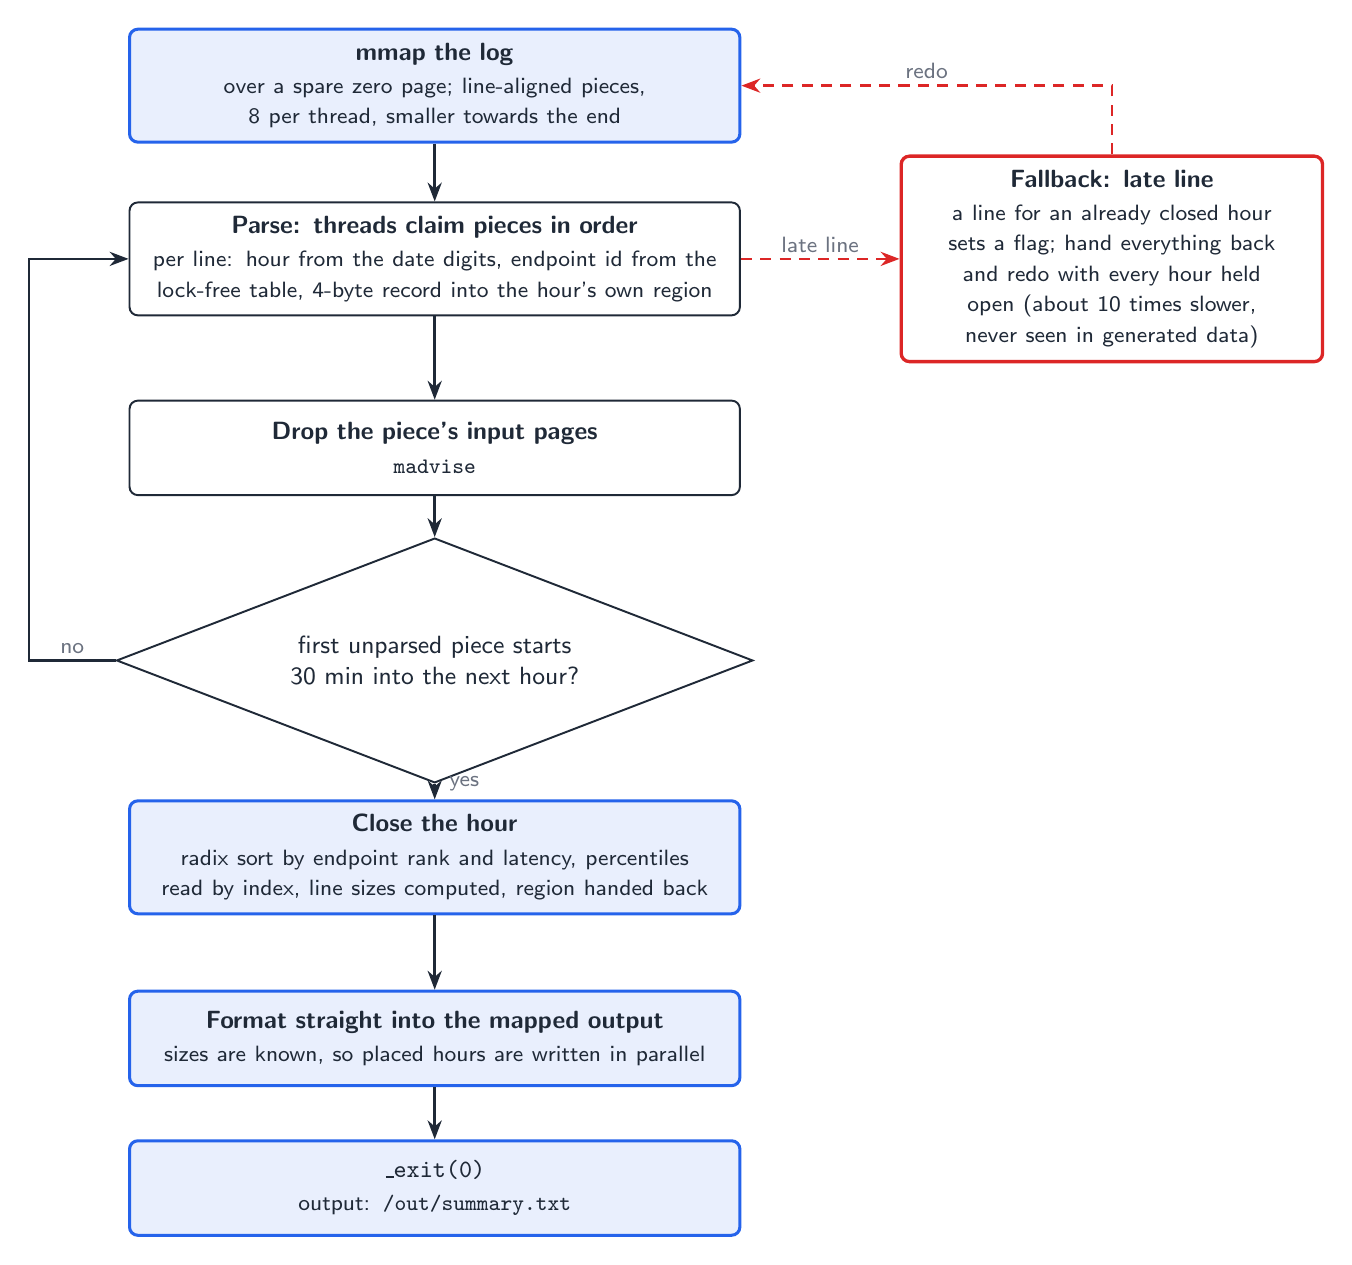
\begin{tikzpicture}
  \def\w{74mm}
  \node[box=\w, hl=cA] (m) at (0,0) {\nt{mmap the log}{over a spare zero page; line-aligned pieces, 8 per thread, smaller towards the end}};
  \node[box=\w] (p) at (0,-2.2) {\nt{Parse: threads claim pieces in order}{per line: hour from the date digits, endpoint id from the lock-free table, 4-byte record into the hour's own region}};
  \node[box=\w] (d) at (0,-4.6) {\nt{Drop the piece's input pages}{\texttt{madvise}}};
  \node[dec=60mm] (q) at (0,-7.3) {first unparsed piece starts 30 min into the next hour?};
  \node[box=\w, hl=cA] (c) at (0,-9.8) {\nt{Close the hour}{radix sort by endpoint rank and latency, percentiles read by index, line sizes computed, region handed back}};
  \node[box=\w, hl=cA] (w) at (0,-12.1) {\nt{Format straight into the mapped output}{sizes are known, so placed hours are written in parallel}};
  \node[box=\w, hl=cA] (x) at (0,-14.0) {\nt{\texttt{\_exit(0)}}{output: \texttt{/out/summary.txt}}};

  \node[box=50mm, accent=warn, draw=warn] (l) at (8.6,-2.2) {\nt{Fallback: late line}{a line for an already closed hour sets a flag; hand everything back and redo with every hour held open (about 10 times slower, never seen in generated data)}};

  \draw[arr] (m) -- (p);
  \draw[arr] (p) -- (d);
  \draw[arr] (d) -- (q);
  \draw[arr] (q) -- node[lab, right, xshift=1mm, yshift=1mm] {yes} (c);
  \draw[arr] (c) -- (w);
  \draw[arr] (w) -- (x);
  \draw[arr] (q.west) -- ++(-1.1,0) node[lab, above, pos=0.5] {no} |- (p.west);
  \draw[redo] (p.east) -- node[lab, above] {late line} (l.west);
  \draw[redo] (l.north) |- node[lab, above, pos=0.75] {redo} (m.east);
\end{tikzpicture}
\end{document}
